%% ----------------------------------------------------------------
%% Chapter_3.tex
%% ----------------------------------------------------------------
\chapter{Project Planning}
\label{Chapter:Planning}

\section{Overview}
Project planning defines the structured roadmap for the development and
completion of EduFeedback AI. The planning process focuses on dividing the
project into well-defined phases to ensure systematic progress, effective time
management, and clear deliverables at each stage. The project is planned across
multiple academic semesters, allowing gradual development, validation, and
refinement of system components.

\begin{longtable}{|l|p{4cm}|p{8cm}|}
    \caption{Phases of the entire project work}
    \label{tab:project_phases} \\
    \hline
    \textbf{Phase} & \textbf{Module Name} & \textbf{Tasks / Implementation Steps} \\
    \hline
    \endfirsthead

    \multicolumn{3}{c}{\small\itshape (Table \ref{tab:project_phases} continued from previous page)} \\
    \hline
    \textbf{Phase} & \textbf{Module Name} & \textbf{Tasks / Implementation Steps} \\
    \hline
    \endhead

    \hline
    \multicolumn{3}{r}{\small\itshape Continued on next page\ldots} \\
    \endfoot

    \hline
    \endlastfoot

    Phase 1 & Alumni Career Outcome Collection System &
    \textbullet\ Design alumni registration/login portal \newline
    \textbullet\ Create structured online survey (job role, skills used, relevance rating, satisfaction) \newline
    \textbullet\ Enable option to update career progress (job change / skill growth)
    \\ \hline

    Phase 2 & Teacher Feedback System \& CO Attainment Analyzer &
    \textbullet\ Develop teacher login panel \newline
    \textbullet\ Create digital feedback form mapped to course outcomes (COs) \newline
    \textbullet\ Allow uploading CO attainment reports \newline
    \textbullet\ Convert teacher feedback into structured database format
    \\ \hline

    Phase 3 & Job--Curriculum Mapping \& Gap Analysis (AI/NLP Engine) &
    \textbullet\ Collect syllabus/course content (text format) \newline
    \textbullet\ Use NLP (TF-IDF / BERT embeddings) to extract key topics \newline
    \textbullet\ Extract job skill keywords from alumni responses \newline
    \textbullet\ Compare syllabus topics vs job-required skills \newline
    \textbullet\ Generate ``Skill Gap Index'' and matching percentage
    \\ \hline

    Phase 4 & AI-Based Recommendation Engine for Curriculum Improvement &
    \textbullet\ Create scoring model to rate relevance of each course \newline
    \textbullet\ Suggest new modules/topics based on missing skills \newline
    \textbullet\ Identify low-ROI topics (taught but not used in job) \newline
    \textbullet\ Generate structured recommendations for syllabus revision
    \\ \hline

    Phase 5 & Visualization \& Decision Support Dashboard &
    \textbullet\ Build interactive dashboard (Streamlit / React + API) \newline
    \textbullet\ Display analytics (graphs, heatmaps, skill gaps) \newline
    \textbullet\ Provide admin panel for HoD/IQAC/NAAC reviewers \newline
    \textbullet\ Enable export to PDF/Excel reports
    \\ \hline

    Phase 6 & Testing \& Validation &
    \textbullet\ Test data consistency across teacher + alumni sheets \newline
    \textbullet\ Validate skill mapping via sample career datasets \newline
    \textbullet\ Pilot use with small group of students/alumni \newline
    \textbullet\ Perform usability testing and feedback review
    \\ \hline

    Phase 7 & Documentation \& Report Preparation &
    \textbullet\ Create project documentation (SRS, DFD, UML) \newline
    \textbullet\ Prepare final presentation PPT + demo video \newline
    \textbullet\ Draft research methodology section
    \\

\end{longtable}

The planning approach emphasizes requirement clarity, modular development,
and incremental implementation, ensuring that the system remains adaptable to
future enhancements and institutional requirements.

\section{Database Design and Data Collection Work}
The database forms the foundation of the EduFeedback AI system, as all analytical insights depend on the quality and structure of the collected data. The primary objective of the database design is to store alumni career information, curriculum relevance feedback, and employability-related attributes in a structured and analyzable format.

\subsection{Data Source and Collection Method}
The data used in this project was collected through a structured online alumni feedback survey. The survey was designed to capture both quantitative and qualitative information related to graduates' academic background, employment status, job roles, skills, and curriculum relevance.

A total of 98 alumni responses were collected at the current stage, covering graduates from different departments, degree programs, and graduation years. The collected data represents real-world employability outcomes and serves as a reliable dataset for curriculum and skill gap analysis.

\begin{figure}[!h]
    \centering
    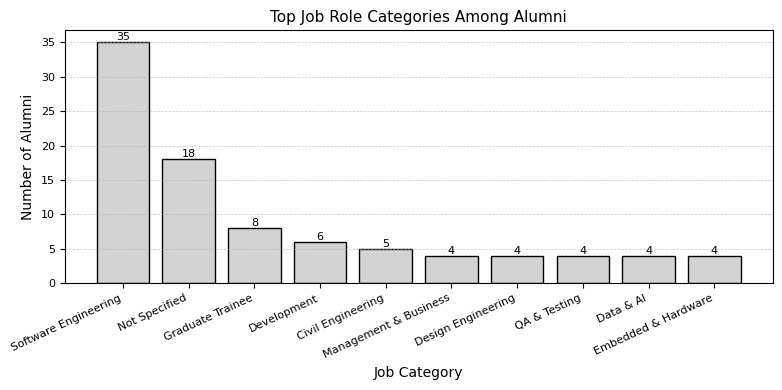
\includegraphics[width=0.7\linewidth]{figures/Chapter_3_Fig/job_distribution.png}
    \caption{Distribution of top job roles among alumni respondents}
    \label{fig:job_roles}
\end{figure}

The figure shows the distribution of job roles among 98 alumni respondents. Machine Learning Engineer has the highest representation, followed by AI Engineer and Backend Developer roles. This reflects a strong trend towards data-driven and software development careers among graduates.

\subsection{Database Schema Design}
The alumni survey data is stored using a hybrid database design approach. Core authentication and identity attributes are maintained in a normalized Users table, while alumni-specific survey responses are stored in JSON format within the Alumni table. This design provides flexibility in handling survey structures and unstructured text required for NLP-based analytics.

\section{System Architecture of EduFeedback AI}
EduFeedback AI follows a layered architecture to ensure modularity, scalability, and ease of maintenance. The system is divided into four logical layers, where each layer performs a specific function and interacts with adjacent layers.

The presentation layer provides role-based access through three interfaces: Alumni Portal, Faculty Portal, and Admin Panel. Alumni submit career details and feedback, faculty members provide course outcome attainment and academic inputs, while administrators monitor analytics and reports.

The application layer acts as the core processing unit of the system. It handles role-based logins, authentication and authorization, and exposes RESTful APIs for communication between the presentation layer and backend services.

The data analytics layer is responsible for intelligence-driven processing. It performs natural language processing using techniques such as TF-IDF and BERT, supports skill-to-curriculum mapping, calculates skill gap indices, and generates recommendations for curriculum improvement.

The data layer consists of a relational SQL database that stores alumni records, feedback data, user credentials, and analysis results. This layer ensures secure and persistent storage of all system data.

\begin{figure}[!h]
    \centering
    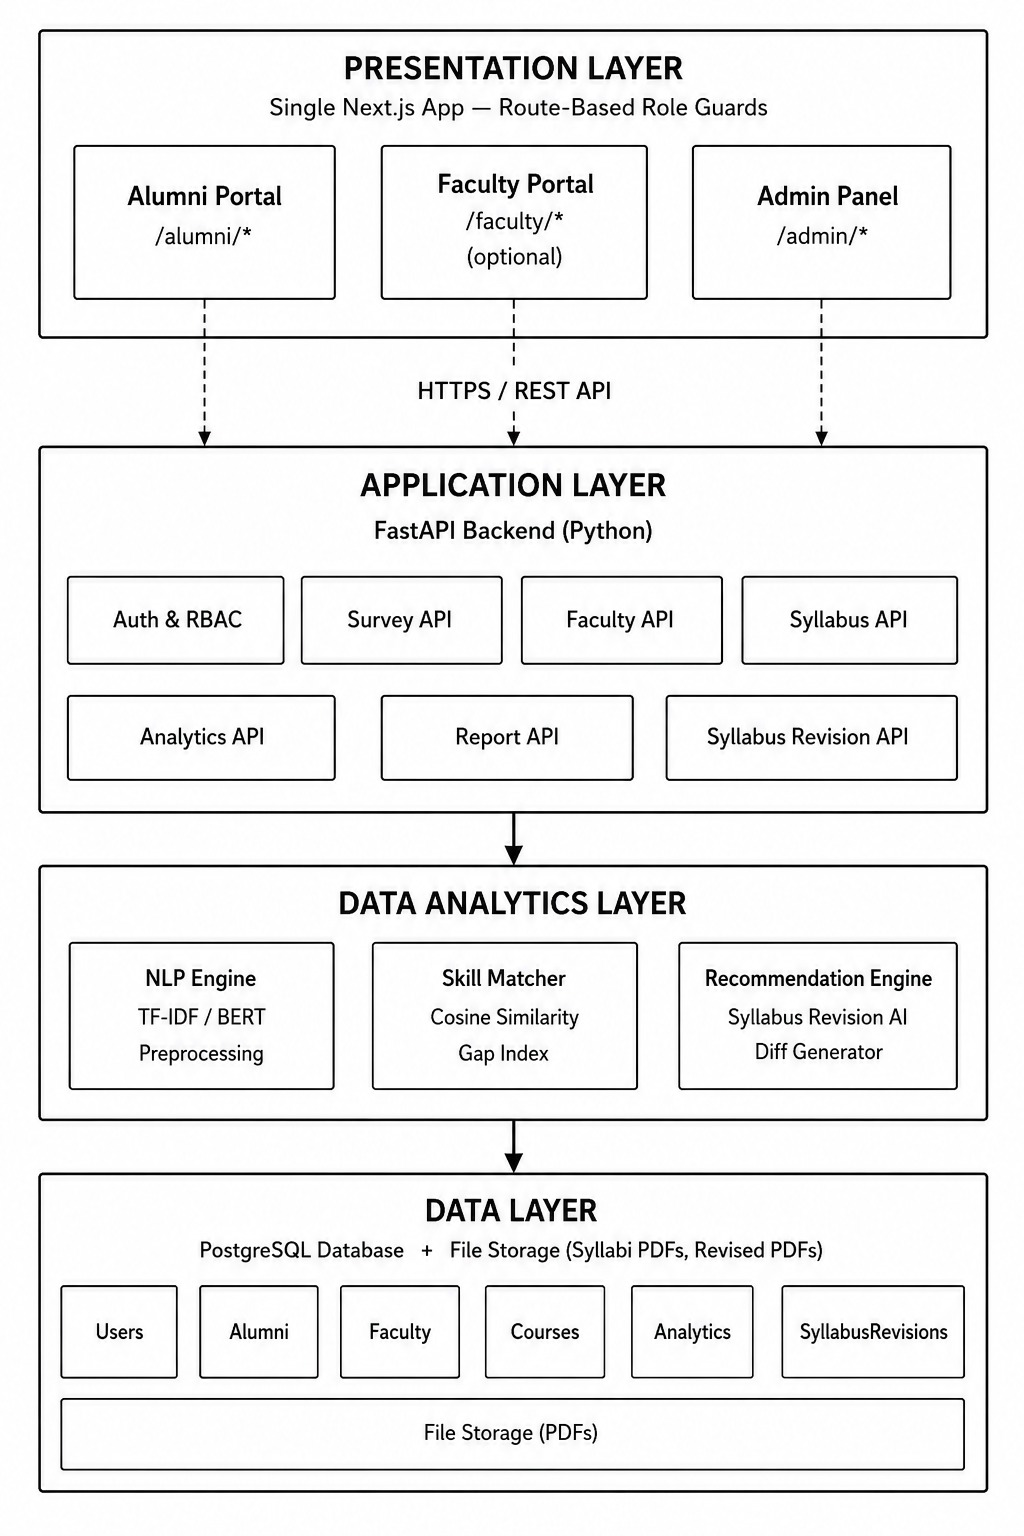
\includegraphics[width=0.7\linewidth]{figures/Chapter_3_Fig/system_architecture.png}
    \caption{System architecture of EduFeedback AI}
    \label{fig:system_architecture}
\end{figure}

\section{Identified Challenges and System Limitations}
During the planning and initial development phase, several challenges and limitations were identified:
\begin{itemize}
    \item Limited volume of alumni responses during early stages
    \item Variability in feedback quality and level of detail
    \item Difficulty in directly mapping academic subjects to diverse job roles
    \item Dependence on voluntary participation for data collection
\end{itemize}

These factors may affect the accuracy and depth of analytical results if not addressed adequately.

\section{Strategy to Address Identified Loopholes}
To mitigate the identified challenges, the following strategies are proposed:
\begin{itemize}
    \item Gradual expansion of alumni participation through structured outreach
    \item Combination of objective questions with descriptive feedback fields
    \item Standardization of skill and subject keywords to improve mapping accuracy
    \item Incremental refinement of analysis techniques as data volume increases
\end{itemize}

These measures are intended to improve data consistency, analytical reliability, and overall system effectiveness.

\section{Project Scheduling and Gantt Chart}
The project schedule is represented using a Gantt chart to illustrate the timeline and sequencing of activities across the project duration. Each phase is mapped to specific time periods, with certain tasks overlapping to ensure efficient utilization of time and timely completion of deliverables.

\begin{figure}[!htbp]
    \centering
    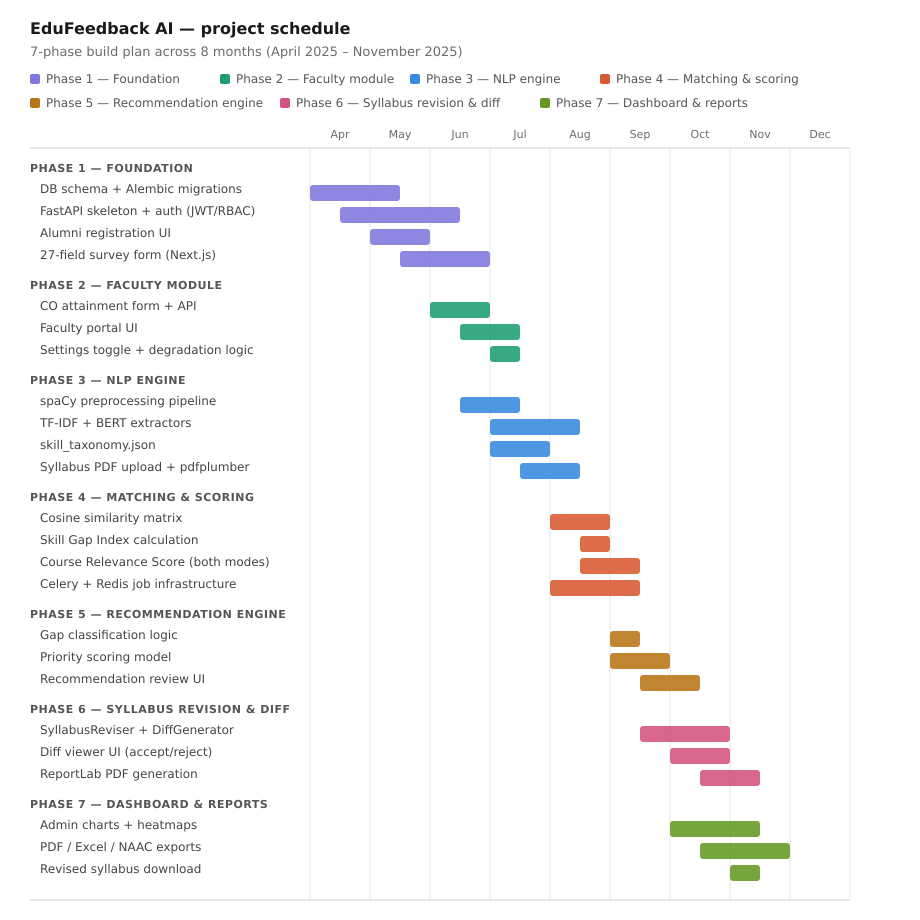
\includegraphics[width=\linewidth, height=0.85\textheight, keepaspectratio]{figures/Chapter_3_Fig/gantt_chart.png}
    \caption{Gantt chart of project schedule}
    \label{fig:gantt_chart}
\end{figure}
